%% Copyright 2018 H.\ Rabus
%
% This work may be distributed and/or modified under the
% conditions of the LaTeX Project Public License, either version 1.3
% of this license or (at your option) any later version.
% The latest version of this license is in
%   http://www.latex-project.org/lppl.txt
% and version 1.3 or later is part of all distributions of LaTeX
% version 2005/12/01 or later.
%
% This work has the LPPL maintenance status `author-maintained'.
%
% This work consists of the file texbsp.tex
%

\documentclass[smallheadings]{scrartcl}

%%% GENERAL PACKAGES %%%%%%%%%%%%%%%%%%%%%%%%%%%%%%%%%%%%%%%%%%%%%%%%%%%%%%%%%%
% inputenc allows the usage of non-ascii characters in the LaTeX source code
\usepackage[utf8]{inputenc}
\usepackage{graphicx} 
\usepackage{float}
%\graphicspath{ {/u/hnatiuka/Praktikum/PPI/} }



% title of the document
\title{Bericht zu Serie 2}
% optional subtitle
%\subtitle{Draft from~\today}
% information about the author
\author{%
  Arsen Hnatiuk,\\%
  Max Huneshagen 
}
\date{\today} 


%%% LANGUAGE %%%%%%%%%%%%%%%%%%%%%%%%%%%%%%%%%%%%%%%%%%%%%%%%%%%%%%%%%%%%%%%%%%
% babel provides hyphenation patterns and translations of keywords like 'table
% of contents'
\usepackage[ngerman]{babel}

%%% HYPERLINKS %%%%%%%%%%%%%%%%%%%%%%%%%%%%%%%%%%%%%%%%%%%%%%%%%%%%%%%%%%%%%%%%
% automatic generation of hyperlinks for references and URIs
\usepackage{hyperref}

%%% MATH %%%%%%%%%%%%%%%%%%%%%%%%%%%%%%%%%%%%%%%%%%%%%%%%%%%%%%%%%%%%%%%%%%%%%%
% amsmath provides commands for type-setting mathematical formulas
\usepackage{amsmath}
% amssymb provides additional symbols
\usepackage{amssymb}
% HINT
% Use http://detexify.kirelabs.org/classify.html to find unknown symbols!

%%% COLORS %%%%%%%%%%%%%%%%%%%%%%%%%%%%%%%%%%%%%%%%%%%%%%%%%%%%%%%%%%%%%%%%%%%%
% define own colors and use colored text
\usepackage[pdftex,svgnames,hyperref]{xcolor}

%%% Code Listings %%%%%%%%%%%%%%%%
% provides commands for including code (python, latex, ...)
\usepackage{listings}
\definecolor{keywords}{RGB}{255,0,90}
\definecolor{comments}{RGB}{0,0,113}
\definecolor{red}{RGB}{160,0,0}
\definecolor{green}{RGB}{0,150,0}
\lstset{language=Python, 
        basicstyle=\ttfamily\small, 
        keywordstyle=\color{keywords},
        commentstyle=\color{comments},
        stringstyle=\color{red},
        showstringspaces=false,
        identifierstyle=\color{green},
        }


\usepackage{paralist}
\usepackage{nicefrac}
% setting the font style for input und returns in description items
\newcommand{\initem}[2]{\item[\hspace{0.5em} {\normalfont\ttfamily{#1}} {\normalfont\itshape{(#2)}}]}
\newcommand{\outitem}[1]{\item[\hspace{0.5em} \normalfont\itshape{(#1)}]}
\newcommand{\bfpara}[1]{
	
	\noindent \textbf{#1:}\,}


\begin{document}

% generating the title page
\maketitle
% generating the table of contents (requires to run pdflatex twice!)
\tableofcontents
\bigskip

\hrule
\hrule

%%% BEGIN OF CONTENT %%%%%%%%%%%%%%%%%%%%%%%%%%%%%%%%%%%%%%%%%%%%%%%%%%%%%%%%%%

\section{Einleitung}

%TODO 
Das analytische Lösen von partiellen Differentialgleichungen kann manchmal schwierig, und oft unmöglich sein.

\section{Theorie}

\subsection{Speicherplatzbedarf}
\label{sec:bedarf}
Der wesentliche Unterschied zwischen vollbesetzten und \textit{sparse}-Matrizen  liegt in dem Speicherbedarf. Während eine vollbesetzte Matrix alle Einträge wie in einem Array speichert, werden nur die nicht-Null Einträge in einer \textit{sparse}-Matrix gespeichert. Also braucht eine $n \times n$ \textit{numpy.matrix} $n^2$ \textit{float}-Speicherplätze, jeweils \textit{64-bit}. Ein \textit{scipy.sparse.dok\_matrix}-Objekt  ist ein Wörterbuch-Objekt, dessen Schlüssel die \textit{(Zeile, Spalte)}-Koordinaten, und dessen Werte die Matrixeinträge sind. Also brauchen $n$ nicht-Null Einträge $2n$ \textit{int}Speicherplätze (für die zwei Schüssel-\textit{arrays}), jeweils \textit{24-bit}, und $n$ \textit{float}-Speicherplätze für den Matrixeintrag. Dagegen sind Keine Null Einträge gespeichert, also enthält das Wörterbuch die Schlüssel mit den Koordinaten der Null Einträge. Ein solches Objekt benutzt auch einen konstanten (also vernachlässigbaren) Speicherplatz für die Dimensionen der Matrix. Wir wenden nun die Speicherbedarfsanalyse auf eine Matrix wie in der Aufgabestellung mit Feinheit der Diskretisierung $n$ an. Wir approximieren dabei der Übersicht halber $2 \cdot 24 \approx 64$, um einen Wörterbuch-Eintrag als zwei \textit{float}-Einträge zu betrachten, damit nut \textit{float}-Speicherplätze in Frage kommen.

\paragraph{d = 1}
In der ersten Dimension hat die vollbesetzte Matrix $n^2$ Einträge, also einen Speicherbedarf der Ordnung $\mathcal{O}(n^2)$.

Die nicht-Null Einträge dieser Matrix stehen auf der drei zentralen Diagonalen. Also benötigt das \textit{scipy.sparse.dok\_matrix}-Objekt $2(n+2(n-1)) = \mathcal{O}(6n)$ Speicherplätze.

\paragraph{d = 2}
Die $d=2$-Matrix besteht aus $n^2$ Matrizen, die die gleiche Größe wie eine $d=1$-Matrix haben. Also ist der Speicherbedarf der \textit{numpy}-Matrix der Ordnung $\mathcal{O}(n^4)$.

 Diese Matrix hat $n$ viele $d=1$-Matrizen auf der Hauptdiagonale  und $2(n-1)$ Einheitsmatrizen auf den zwei Nebendiagonalen, mit jeweils $n$ nicht-Null Einträge. Insgesamt macht das $2(n(\mathcal{O}(6n))+2n(n-1))=\mathcal{O}(16n^2)$ Speicherplätze.
 
 \paragraph{d = 3}
 Die $d=3$-Matrix besteht aus $n^2$ Matrizen, die die gleiche Größe wie eine $d=2$-Matrix haben. Also ist der Speicherbedarf der \textit{numpy}-Matrix der Ordnung $\mathcal{O}(n^6)$.
 
 Die untersuchte Matrix hat $n$ viele $d=2$-Matrizen auf der Hauptdiagonale  und $2(n-1)$ Einheitsmatrizen auf den zwei Nebendiagonalen, mit jeweils $n^2$ nicht-Null Einträge. Insgesamt macht das $2(n(\mathcal{O}(16n^2))+2n^2(n-1))=\mathcal{O}(36n^3)$ Speicherplätze.


\subsection{Lineares Gleichungssystem}

Die zentrale Problematik, zum Lösen von welchen die implementierte Python-Klasse dient, ist das Lösen der partiellen Differentialgleichung

\begin{align}
-\Delta u=f(x)
\end{align}
auf einem Gebiet $\Omega=(0, 1)^d$ für $d\in \{1, 2, 3\}$ für ein gegebenes $f$ und für Randbedingungen $u_D \in \partial\Omega$, wobei 
\begin{align}
\Delta u=\sum_{j=1}^{d}\frac{\partial^2 u}{\partial x_j^2}
\end{align}

Wir wollen $u$ approximieren, und dafür benutzen wir die aus der Serie 1 bekannte Abschätzung
\begin{align}
\frac{\partial^2 u}{\partial x_j^2}(x)=\frac{u(x-e_jh)+u(x+e_jh)-2u(x)}{h^2}+\mathcal{O}(h^2)
\label{eq:diff}
\end{align} 
Da es unmöglich ist, dies numerisch für jeden Punkt in $\Omega$ zu berechnen, wählen wir nur eine endliche Menge von Punkten. Dafür machen wir eine Diskretisierung des Definitionsbereichs. 

\paragraph{ Dsikretisierung}

Wir Zerlegen den Definitionsbereich mithilfe eines uniformen Gitters mit Schrittweite $h = 1/n$. Die Schnittpunkte auf diesem Gitter sind dann die Punkte, auf den die Funktion $u$ zu approximieren ist. Sei $P$ die Menge dieser Punkte. Für $d=3$ hat jeder Punkt $x\in P$ die Gestalt $x = (\frac{i}{n}, \frac{j}{n}, \frac{k}{n})$ für natürliche Zahlen $i, j, k \leq n$. Entsprechend gilt für $d=2$ $x=(\frac{i}{n}, \frac{j}{n})$ und für $d=1$ $x=(\frac{i}{n})$.
Damit wir mit diesen Punkten arbeiten können, ist es sehr günstig, sie durchzunummerieren, anstelle davon, mehrere Indizes zu haben. Für $d=1$ erfolgt dies ganz intuitiv - wir nummerieren die Punkte nach Position, also $x_i = (\frac{i}{n})$. Für die höheren Dimensionen wollen wir, dass die Nummerierung erstens in der $i$-Richtung, zweitens in der $j$-Richtung und letztens in der $k$-Richtung erfolgt. Dafür führen wir die folgende Funktion ein:
\begin{align}
g(m)=
\begin{cases} 
n-1 &m\mod{n-1} \\
m\mod{n-1} & sonst \\
\end{cases}
\end{align}
Die Nummerierungen für $d=2$ und $d=3$ sehen also so aus: 
\begin{align}
x_m=(\frac{g(m)}{n},\frac{\ulcorner\frac{m}{n}\urcorner}{n} ) 
\end{align}
Beziehungsweise
\begin{align}
x_m=(\frac{g(m)}{n}, \frac{g(\ulcorner\frac{m}{n}\urcorner)}{n}, \frac{\ulcorner\frac{m}{(n-1)^2+1}\urcorner}{n}) 
\end{align}
wobei $\ulcorner \cdot \urcorner$ eine Rundung nach oben bezeichnet. Nach dieser Rechenvorschrift wird jedem $m$ zwischen 1 und $(n-1)^d$ ein eindeutiges Punkt zugewiesen. Man sieht auch: für $x_m = (\frac{i}{n}, \frac{j}{n}, \frac{k}{n})$ gilt $x_{m\pm(n-1)} = (\frac{i}{n}, \frac{j\pm1}{n}, \frac{k}{n})$ und $x_{m\pm(n-1)^2} = (\frac{i}{n}, \frac{j}{n}, \frac{k\pm1}{n})$
 Nun können wir die Formel \eqref{eq:diff} auf diesen Punkten anwenden.

\paragraph{Diskretisierung der Differentialgleichung}
Die Formel \eqref{eq:diff} lässt sich unter Vernachlässigung von $\mathcal{O}(h^2)$ so schreiben:
\begin{align}
f(x) = \frac{-u(x-e_1h)-u(x+e_1h)-u(x-e_2h)+u(x+e_2h)-u(x-e_3h)+u(x+e_3h)+2du(x)}{h^2}
\end{align}
Wenn wir $h$ wie im letzten Absatz auffassen, können wir die Formel bezüglich der Punkte in $P$ mit der Eigenschaft $x_m=(\frac{i}{n}, \frac{j}{n}, \frac{k}{n})$, $i, j, k \notin \{1, (n-1)\}$ (sei $P*$ die Menge dieser Punkte) und die darauf definierte Nummerierung darstellen:
\begin{align}
f(x_m) = \frac{-\hat{u}(x_{m-1})-\hat{u}(x_{m+1})-\hat{u}(x_{m-(n-1)})+\hat{u}(x_{m+(n-1)})-\hat{u}(x_{m-(n-1)^2})+\hat{u}(x_{m+(n-1)^2})+2d\hat{u}(x)}{h^2}
\label{eq:diff2}
\end{align}
wobei $\hat{u}$ eine Approximation von $u$ ist (wir haben einen Fehler der Ordnung $\mathcal{O}(h^2)$ vernachlässigt), und die Terme $x_{m\pm(n-1)}$ und $x_{m\pm(n-1)^2}$ für $d=1$ und $x_{m\pm(n-1)^2}$ für $d=2$	verschwinden. Aus der Definition der gewählten Nummerierung sieht man, dass die Formel \eqref{eq:diff2} dem linearen Gleichungssystem $A_{P*}\hat{u}=b_{P*}$ entspricht, wobei $A_{P*}$ die Matrix aus Teil 1, aber ohne die Zeilen, die zu den $x_m \in P\setminus P*$ entsprechen, und  $b_{P*}$ - der Vektor, von $f(x_m)$, aber wieder ohne die $x_m \in P\setminus P*$.

\paragraph{Aufstellen des linearen Gleichungssystems}

Damit wir das lineare Gleichungssystem für alle $x_m$ aufstellen können, müssen die Randbedingungen $u_D \in \partial\Omega$ berücksichtigt werden, weil die Punkte $x \pm e_jh$ nicht immer in $P$ liegen. In den Matrizen aus Teil 1 werden diese Einträge nicht berücksichtigt, also damit wir das Gleichungssystem als $A\hat{u}=b$ schreiben können, müssen wir $b_P$ (der Vektor mit Einträgen $f(x_m)$ für $m \in P$) mit den Termen aus dem Rand $\partial\Omega$ vervollständigen. 
Sei $b_i :=f(x_i)$. Wir erweitern nun diese Werte.  

Für $m = k(n-1)+1$ mit ein $k \in \mathbb{N}\cup \{0\}$ setze man $b_m = b_m + \frac{u(x_m - e_ih)}{h^2}$. Für $m = k(n-1) +1$ mit ein $k \in \mathbb{N}$ setze man $b_m = b_m + \frac{u(x_m + e_ih)}{h^2}$. Man mache dies für $d\in \{1, 2, 3\}$.

Für $m \in (k(n-1)^2+1, k(n-1)^2+n-1)$ mit ein $k \in \mathbb{N}\cup \{0\}$ setze man $b_m = b_m + \frac{u(x_m)-e_jh}{h^2}$. Für $m \in (k(n-1)^2-(n-1), k(n-1)^2-1)$ mit ein $k \in \mathbb{N}$ setze man $b_m = b_m + \frac{u(x_m)+e_jh}{h^2}$.  Man mache dies für $d\in \{2, 3\}$.

Für $m\in (1, (n-1)^2)$ setze man $b_m = b_m + \frac{u(x_m-e_kh)}{h^2}$. Für $m\in ((n-1)^3-(n-2), (n-1)^3)$ setze man $b_m = b_m + \frac{u(x_m+e_kh)}{h^2}$.  Man mache dies für $d=3$.

Nach diese Umformungen können wir das Modell zur Approximierung der partiellen Differentialgleichung als $A\hat{u}=b$ schreiben.

\section{Experimente}

In \textit{experimente.py} wird die relative Anzahl der Nicht-Null-Einträge der Matrix $A^{(d)}$ für $d=1,2,3$ numerisch untersucht und anschließend graphisch dargestellt. Darüber hinaus wird die Gesamtanzahl der Einträge einer vollbesetzen Matrix der gleichen Größe wie $A^{(d)}$ in Abhängigkeit von $n$ geplottet. Diese ergibt sich zu $(n-1)^{2d}$, da $A^{(d)}\in\mathbb{R}^{(n-1)^d\times(n-1)^d}$ Das Ergebnis des Experiments ist in Abb.~\ref{im:nn_eintr} doppeltlogarithmisch dargestellt.

\begin{figure}[H]
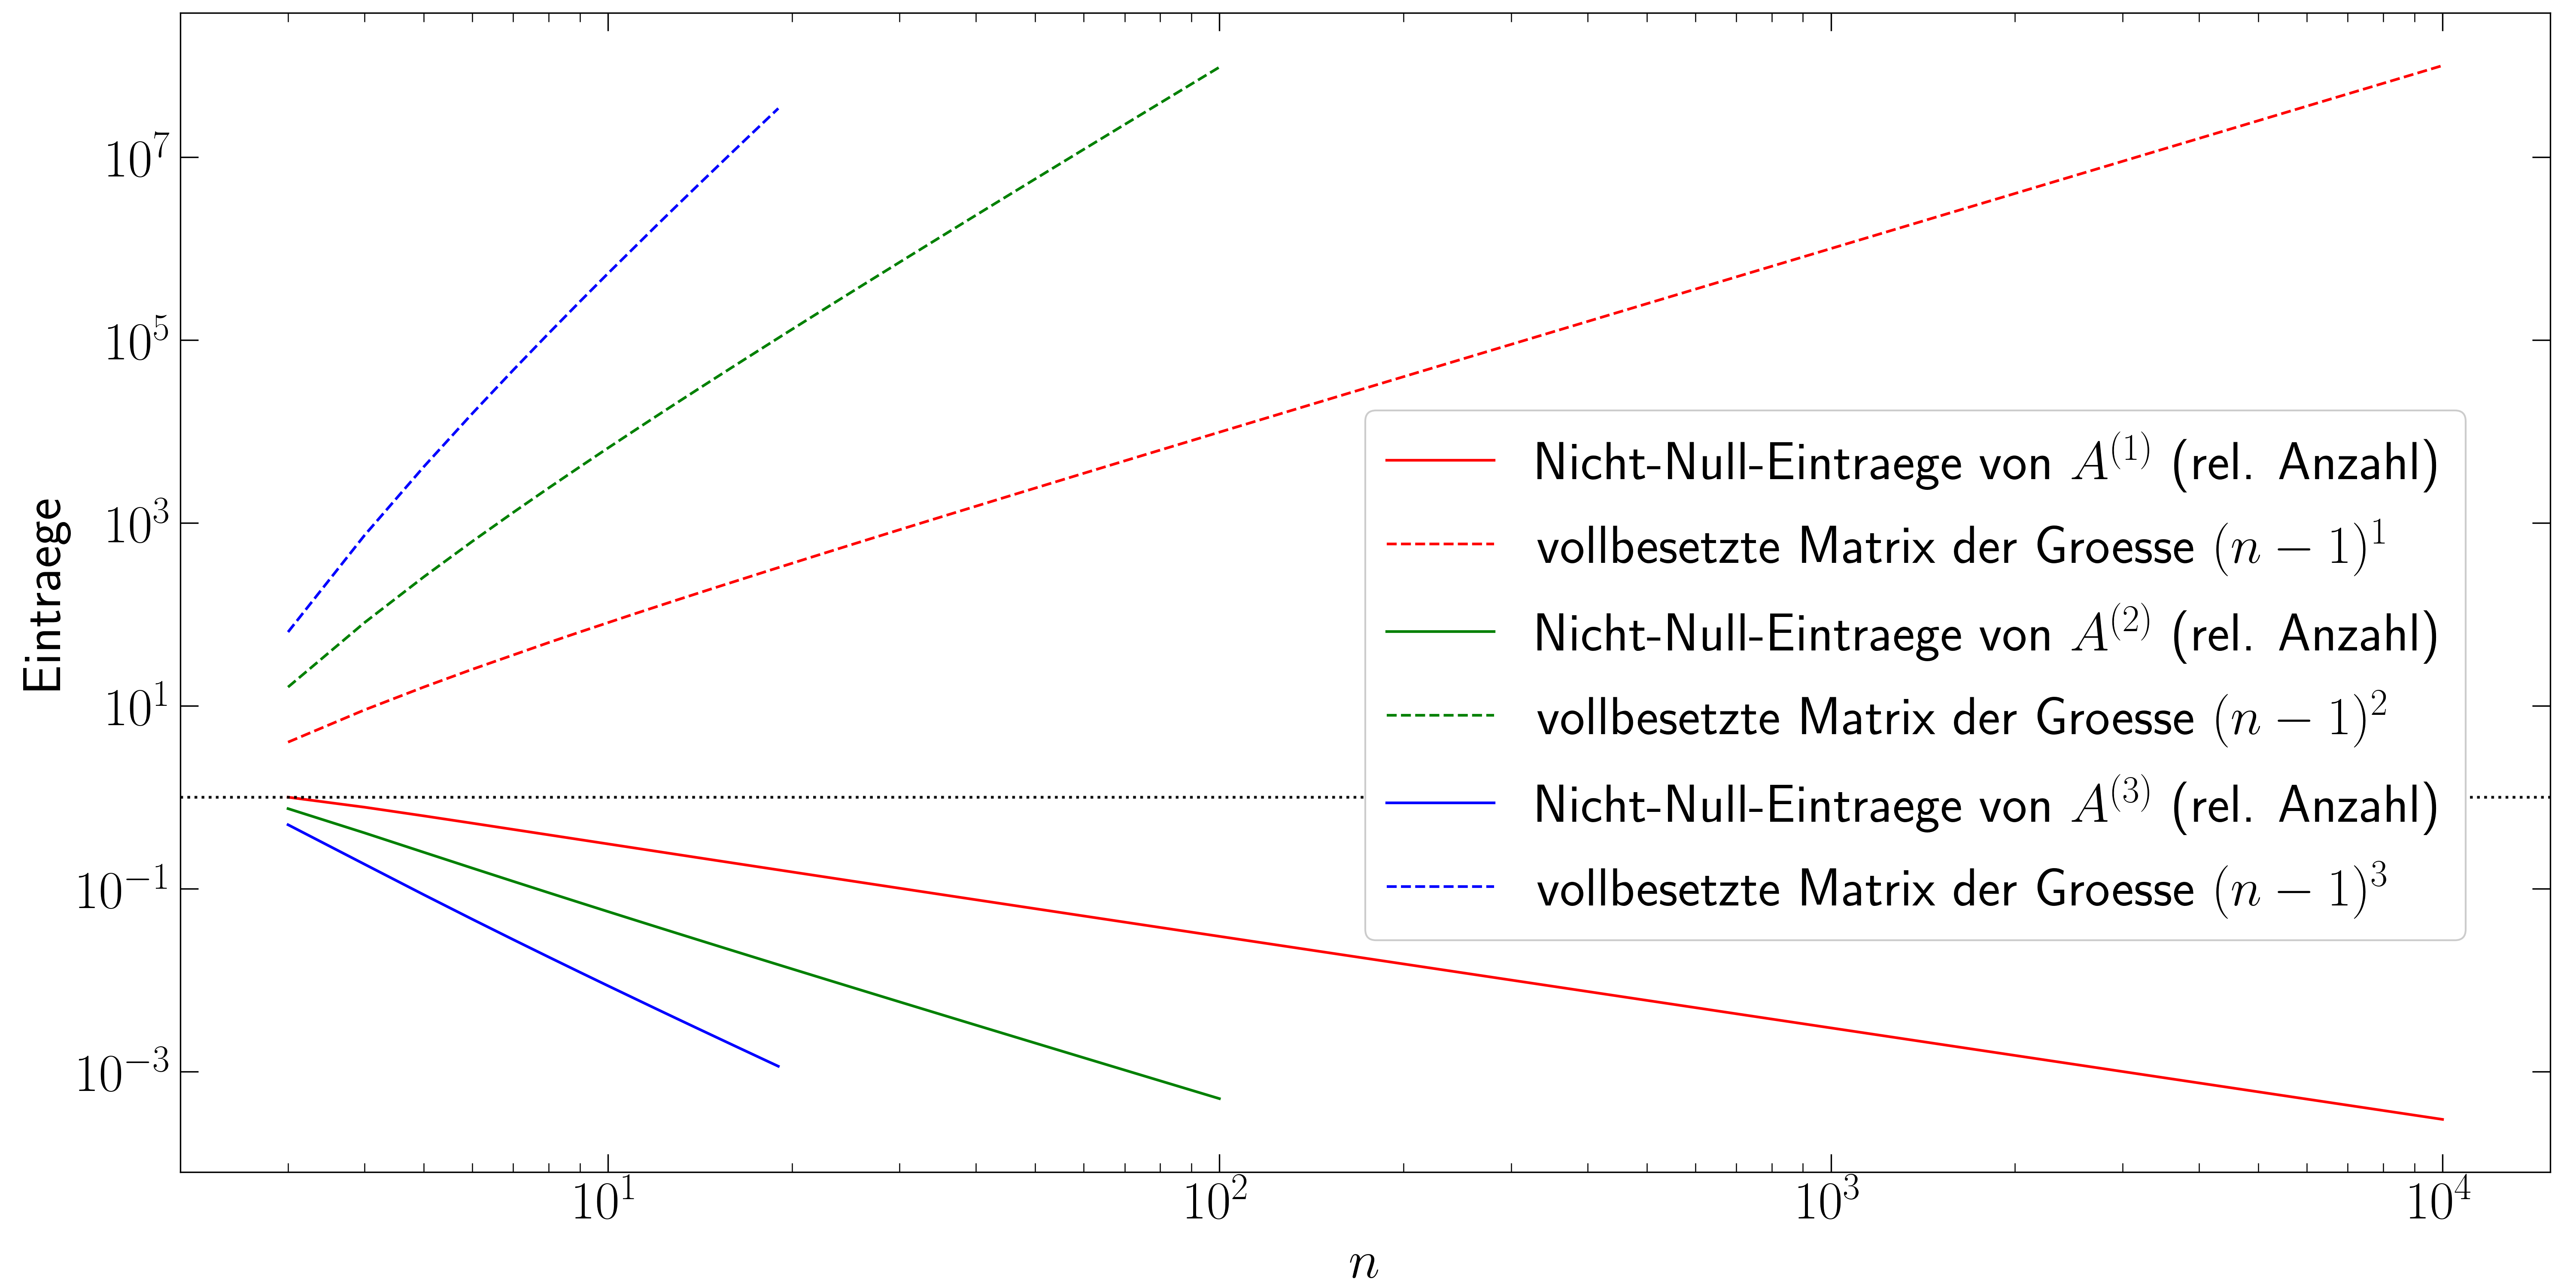
\includegraphics[width=\textwidth]{Bilder/nn_eintraege}

\caption{Durchgezogen: Nicht-Null-Einträge von $A^{(d)}$ für $d=1,2,3$ (relative Anzahl). Gestrichelt: Einträge einer vollbesetzten Matrix der gleichen Größe wie $A^{(d)}$.}
\label{im:nn_eintr}
\end{figure}



Man erkennt, dass die relative Anzahl der Nicht-Null-Einträge (und damit der Speicheraufwand des \textit{scipy.dok\_matrix}-Objektes für jedes untersuchte $d$ verschieden stark abfällt. Bezeichnet $a_{\text{nn},d}(n)$ die Anzahl der 
Nicht-Null-Einträge von $A^{(d)}$, so ergibt sich durch eine graphische Analyse, dass $a_{\text{nn},d}\sim n^{-d}$ wie in Abschnitt \ref{sec:bedarf} vorhergesagt. Mit zunehmender Feinheit der Diskretisierung wird die Matrix deutlich dünner besetzt und die Speicherung als Sparse-Matrix immer sinnvoller. Man beachte dazu insbesondere die zunehmende Differenz zum Wert 1, der in Abb.~\ref{im:nn_eintr} durch eine gepunktete Linie eingetragen wurde. 


\section{Zusammenfassung}


\begin{thebibliography}{9}
\bibitem{wiki} Kein Autor, Aufgerufen am 22.11.2018, \textit{Sparse Matrix}. 
\url{https://en.wikipedia.org/wiki/Sparse_matrix}
\end{thebibliography}


%%% END OF DOCUMENT %%%%%%%%%%%%%%%%%%%%%%%%%%%%%%%%%%%%%%%%%%%%%%%%%%%%%%%%%%%
\end{document}
